\documentclass[3p,twocolumn]{elsarticle}
\usepackage{amsmath}
\usepackage{amssymb}
\usepackage{amsmath}
\usepackage{color}
\usepackage{hyperref}
\journal{Computer Physics Communications}
%\journal{The Onion}

\begin{document}

\begin{frontmatter}

\title{Continuous-Time Quantum Monte Carlo Impurity Solvers}

\author[columbia]{Emanuel Gull} \ead{gull@phys.columbia.edu}
\author[eth]{Philipp Werner} \ead{werner@itp.phys.ethz.ch}
\author[goettingen]{Sebastian Fuchs} \ead{fuchs@theorie.physik.uni-goettingen.de}
\author[eth]{Brigitte Surer} \ead{surerb@itp.phys.ethz.ch}
\author[goettingen]{Thomas Pruschke} \ead{pruschke@theorie.physik.uni-goettingen.de}
\author[eth]{Matthias Troyer}\ead{troyer@itp.phys.ethz.ch}

\address[columbia]{Columbia University, New York, NY 10027, USA}
\address[eth]{ETH Zurich, 8093 Zurich, Switzerland}
\address[goettingen]{Georg-August-Universit\"{a}t G\"{o}ttingen, G\"{o}ttingen, Germany}

\begin{abstract}
Continuous-time quantum Monte Carlo impurity solvers are algorithms that sample the partition function of an impurity model using diagrammatic Monte Carlo techniques. The present paper describes codes that implement the interaction
expansion algorithm originally developed by Rubtsov, Savkin, and Lichtenstein, as well as the hybridization expansion method developed by Werner, Millis, Troyer, {\it et al.}. These impurity solvers are part of the ALPS-DMFT application package and are accompanied by an implementation of dynamical mean-field self-consistency equations for (single orbital single site) dynamical mean-field problems with arbitrary densities of states.
\end{abstract}

\end{frontmatter}
{\bf PROGRAM SUMMARY}
  %Delete as appropriate.

\begin{small}
\noindent
{\em Manuscript Title:} Continuous-Time Quantum Monte Carlo Impurity Solvers \\ 
{\em Authors:} Emanuel Gull, Philipp Werner, Sebastian Fuchs, Brigitte Surer, Thomas Pruschke, Matthias Troyer\\ 
{\em Program Title:} dmft \\
{\em Journal Reference:}                                      \\
  %Leave blank, supplied by Elsevier.
{\em Catalogue identifier:}                                   \\
  %Leave blank, supplied by Elsevier.
{\em Licensing provisions:} Use of `dmft' requires citation of this paper. Use of any ALPS program requires citation of the ALPS \cite{ALPS} paper.\\
{\em Programming language:} \verb*#C++# \\
%{\em Computer:} Any \\ 
  %Computer(s) for which program has been designed.
%{\em Operating system:} Any\\ 
  %Operating system(s) for which program has been designed.
{\em RAM:} 10 MB - 1 GB.\\ 
  %RAM in bytes required to execute program with typical data.
{\em Number of processors used:} 1 - 512.\\ 
  %If more than one processor.
{\em Keywords:} DMFT, CT-QMC, CT-HYB, CT-INT.\\ 
  % Please give some freely chosen keywords that we can use in a
  % cumulative keyword index.
{\em Classification:} 7.3 \\ 
  %Classify using CPC Program Library Subject Index, see (
  % http://cpc.cs.qub.ac.uk/subjectIndex/SUBJECT_index.html)
  %e.g. 4.4 Feynman diagrams, 5 Computer Algebra.
{\em External routines/libraries:}  ALPS \cite{ALPS}, BLAS/LAPACK, HDF5.\\ 
{\em Running time:} 60s --8h per iteration.\\
  %Give an indication of the typical running time here.
\end{small}
%% main text
\section{Introduction: Quantum impurity models and impurity solvers}
Quantum impurity models appear in a variety of contexts and play an important role in the study of correlated electron systems. The impurity model may either represent a nano-structure such as a quantum dot or adatom on a surface, or it may serve as an auxiliary problem whose solution yield the ``dynamical mean field" (DMFT) \cite{Georges96,Pruschke95} description of correlated lattice models. Powerful impurity solvers are in particular required for recently developed extensions of DMFT \cite{Maier05,Rubtsov08} and for the study realistic materials \cite{Kotliar06}.

%Quantum impurity models are of crucial importance in the context of correlated electron systems, where they appear in a wide range of applications, ranging from non-equilibrium nano-systems to auxiliary problems in the context of the so-called ``dynamical mean-field'' theory (DMFT) \cite{Georges96,Pruschke95,Kotliar06} and extensions thereof \cite{Maier05,Rubtsov08}, for the study of model systems and real materials.

Quantum impurity models are amenable to numerical study, and numerous solution techniques exist, among them approximate semi-analytical \cite{Georges92,Keiter71,Pruschke89}, renormalization group \cite{NRGRev}, and quantum Monte Carlo methods. The Hirsch-Fye \cite{Hirsch86} quantum Monte Carlo method, long the method of choice for controlled quantitative studies, has one important disadvantage: it suffers from a Trotter breakup (`$\Delta \tau$') error that, in practice, needs to be controlled by means of extrapolation procedures.
Continuous-time methods, originally developed by Rubtsov {\it et al.} \cite{Rubtsov04,Rubtsov05} and Werner {\it et al.} \cite{Werner06}, and later extended by various authors \cite{Werner06Kondo,Haule07,Gull08_ctaux,Gull10_bold,Assaad10}, are based on partition function expansions that are stochastically sampled to all orders using diagrammatic quantum Monte Carlo techniques \cite{Prokofev98,Prokofev98A}, thereby avoiding such errors.
These methods are orders of magnitude more efficient than Hirsch Fye \cite{Gull07} and have rapidly become the methods of choice for the simulation of quantum impurity models, in particular in the context of the DMFT, where the possibility of treating more complicated interactions (in particular the full multiplet structure of multi-orbital systems \cite{Werner06Kondo} and retardation effects \cite{Assaad07,Werner07holstein}) has allowed access to important new physics.
Recent applications include simulations of model systems, realistic material simulations, as well as ``dual Fermion''\cite{Rubtsov08} and cluster extensions \cite{Gull08_plaquette,Werner098site,Gull09_8site}.

With this paper we provide implementations of continuous-time methods and a DMFT self-consistency framework, with the intention of enabling the reader to develop his own codes based on these programs, as well as supplying the community with state-of-the-art implementations for dynamical mean-field calculations. The implementations are based on version 2.0 of the open source ALPS library \cite{ALPS} available at \href{http://alps.comp-phys.org}{http://alps.comp-phys.org}.

In the remainder of this paper we review quantum impurity models (Sec.~\ref{intro_sec}) and continuous-time algorithms (Sec.~\ref{ctint_sec} and \ref{cthyb_sec}), present the DMFT self-consistency conditions \ref{self_sec}, and guide the reader through some of our examples (Sec.~\ref{examples}).

\section{Continuous-Time Quantum Monte Carlo Impurity Solvers}
\label{intro_sec}
A quantum impurity model represents an atom or molecule (the `impurity') embedded in some host material (the `bath' or `leads') and can be described by a Hamiltonian
\begin{align}\label{eq:imp}
H=H_\text{imp}+H_\text{bath}+H_\text{mix}.
\end{align}
Here, $H_\text{imp}=H_\text{imp}^0+H_\text{imp}^I$ corresponds to the impurity (finite number of degrees of freedom, creation operators $d^\dagger_\alpha$) with non-interacting and interacting parts
%
\begin{eqnarray}
H_\text{imp}^0 &=& \sum_{\alpha\beta} \epsilon_{\alpha\beta} d^\dagger_\alpha d_\beta,\\
H_\text{imp}^I &=& \sum_{\alpha\beta\gamma\delta} U_{\alpha\beta\gamma\delta} d^\dagger_\alpha d^\dagger_\beta d_\gamma d_\delta,
\end{eqnarray} 
%
while $H_\text{bath}$ represents a non-interacting bath (infinite number of degrees of freedom, creation operators $a^\dagger_\nu$)
%
\begin{eqnarray}
H_\text{bath} &=& \sum_{\nu} \epsilon_{\nu} a^\dagger_\nu a_\nu,
\end{eqnarray} 
%
and $H_\text{mix}$ the exchange of electrons between the impurity and the bath (hybridization amplitude $V$),
%
\begin{eqnarray}
H_\text{mix} &=& \sum_{\nu\alpha} V_{\nu}^\alpha a^\dagger_\nu d_\alpha + H. c..
\end{eqnarray} 
%
Continuous-time Quantum Monte Carlo impurity solvers allow the accurate and efficient simulation of impurity models. The methods are based on an expansion of the partition function $Z=\text{Tr}[{\rm e}^{-\beta H}]$ into a series of diagrams and the stochastic sampling of (collections of) these diagrams. In the interaction expansion \cite{Rubtsov04,Rubtsov05}, the Hamiltonian Eq.~(\ref{eq:imp}) is split into a non-interacting part $H_1=H_\text{imp}^0+H_\text{bath}+H_\text{mix}$ and an interacting part $H_2=H-H_1=H_\text{imp}^I$, while for the hybridization expansion \cite{Werner06, Werner06Kondo}, the Hamiltonian is split into the local part $H_1=H_\text{imp}+H_\text{bath}$ and the hybridization part $H_2=H-H_1=H_\text{mix}$. In either case, one then employs the interaction representation in which the time evolution of operators is given by $H_1$: $O(\tau)={\rm e}^{\tau H_1}O {\rm e}^{-\tau H_1}$. Using the imaginary-time-ordering operator $\mathcal{T}_{\tau}$ the partition function can be expressed as a time-ordered exponential, which is then expanded into powers of $H_2$,
%
\begin{align}
Z&=\text{Tr} \Big[{\rm e}^{-\beta H_1} \mathcal{T}_{\tau}{\rm e}^{-\int_0^\beta {\rm d}\tau H_2(\tau)} \Big]\nonumber\\
&=\sum_{n=0}^\infty \int_0^\beta {\rm d}\tau_1\ldots \int_{\tau_{n-1}}^\beta {\rm d}\tau_n \text{Tr}\Big[ {\rm e}^{-(\beta-\tau_n)H_1}(-H_2) \ldots \nonumber \\
&\ldots {\rm e}^{-(\tau_2-\tau_1)H_1}(-H_2){\rm e}^{-\tau_1H_1}\Big].
\label{Z_interaction_picture}
\end{align}
%
Eq.~(\ref{Z_interaction_picture}) represents the partition function as a sum over all configurations $c=\{\tau_1<\ldots<\tau_n\}$, $n=0$, $1$, $\ldots$, $\tau_i\in[0,\beta)$ with weight
$w_c=\text{Tr}[ {\rm e}^{-(\beta-\tau_n)H_1}(-H_2)\ldots {\rm e}^{-(\tau_2-\tau_1)H_1}(-H_2){\rm e}^{-\tau_1H_1}]{\rm d}
\tau^n$ and these configurations are sampled by a Monte Carlo procedure.  

In the following two sections we will describe the interaction and hybridization expansion algorithms in some more detail for the simple case of the single-orbital Anderson Impurity model (AIM) for which ($\sigma$ denotes spin, $n_\sigma=d^\dagger_\sigma d_\sigma$) $H_\text{imp}=-\mu (n_\uparrow+n_\downarrow)+U(n_\uparrow n_\downarrow)$.

\section{Interaction expansion impurity solver CT-INT}
\label{ctint_sec}
The continuous-time impurity solver based on the weak-coupling expansion has been proposed in \cite{Rubtsov05, 
Rubtsov04}. For the single-orbital AIM, the Monte Carlo configurations $c=\{\tau_1<\ldots<\tau_n\}$ correspond to collections of interaction vertices placed at positions $\tau_i$ on the imaginary time interval. The weight of such a configuration is given by 
%
\begin{align}
w_c=(-U{\rm d}\tau)^n \det M,
\end{align}
%
where $M$ is an $n\times n$ matrix with elements $M_{ij}=\mathcal{G}_0(\tau_i-\tau_j)$, and $\mathcal{G}_0(\tau)$ (or its Fourier transform $\mathcal{G}_0({\rm i}\omega_n)$) is the ``bath Green's function'' defined in terms of the bath energy levels $\epsilon_\nu$ and hybridization amplitudes $V_\nu$ as \cite{Georges96}
%
\begin{eqnarray}
\mathcal{G}_0({\rm i}\omega_n) &=& [{\rm i}\omega_n+\mu-\Delta({\rm i}\omega_n)]^{-1},\label{eq:g0}\\
\Delta({\rm i}\omega_n) &=& \sum_\nu \frac{|V_\nu|^2}{{\rm i}\omega_n-\epsilon_\nu}\label{eq:hyb}.
\end{eqnarray}
%
In the case of repulsive interactions the chemical potentials for spin up and down must be shifted to avoid a trivial sign problem arising from the factor $(-U)^n$ \cite{Rubtsov05}.


\section{Hybridization expansion impurity solver CT-HYB}
\label{cthyb_sec}

The continuous-time impurity solver based on the hybridization expansion was developed in \cite{Werner06,Werner06Kondo}. After the expansion of the partition function in powers of $H_2=H_\text{mix}$, the time evolution (given by $H_1$) no longer couples the impurity and the bath. One can thus integrate out the bath degrees of freedom analytically to obtain
%
\begin{align}
w_{\tilde c}=&Z_\text{bath} \nonumber
\text{Tr}_\text{imp} \Big[{\rm e}^{-\beta H_\text{imp}} T_\tau
d^\dagger_{\alpha_n'}(\tau_{n}')d_{\alpha_{n}}(\tau_n)
\ldots \\
&d^\dagger_{\alpha_1'}(\tau_1')d_{\alpha_1}(\tau_1) \Big]\nonumber
\times \det M\Big(\{\tau_1, \alpha_1\},\ldots,\{\tau_{n},\alpha_n\}; \\ 
&\{\tau_1',\alpha_1'\},\ldots,\{\tau_{n}',\alpha_n'\}\Big) ({\rm d}\tau)^{2n}.
\label{weight_strong}
\end{align}
%
A configuration $\tilde c$ corresponding to perturbation order $2n$ thus is a collection of $n$ time arguments $\tau_1<\ldots<\tau_n$ corresponding to annihilation operators with spin indices $\alpha_1, \ldots,\alpha_n$ and $n$ time arguments $\tau_1'<\ldots<\tau_n'$ corresponding to creation operators with spin indices $\alpha_1', \ldots, \alpha_n'$. The element $i,j$ of the matrix $M$ is given by the hybridization function $\Delta(\tau_i'-\tau_j)$ \cite{Werner06Kondo}. 

Up to the irrelevant constant $Z_\text{bath}$ the weights consist of two factors: $\text{Tr}_\text{imp}[\ldots]$ evaluates the imaginary-time evolution of the quantum impurity for a given sequence of hybridization events, while $\det M$ gives the contribution of the bath degrees of freedom which have been integrated out. In the general case the computation of the trace factor will lead to an exponential scaling of the algorithm with number of orbitals. In the AIM and its multi-orbital generalizations with density-density interactions, however, the occupation number basis is an eigenbasis of $H_{\rm imp}$ and thus the very efficient segment formulation \cite{Werner06} may be used. 


\begin{figure}
\centering
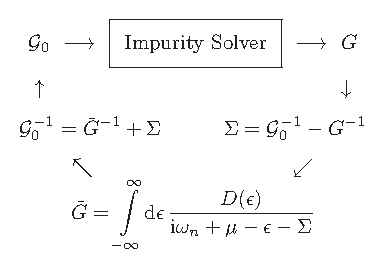
\includegraphics{loop.eps}
\caption{The DMFT self-consistency loop. The dependence of $\Sigma$
  and all Green's functions on the Matsubara frequency ${\rm
    i}\omega_n$ is omitted for simplicity}
\label{fig:loop}
\end{figure}
\section{Dynamical mean-field theory}
\label{self_sec}
The dynamical mean-field theory (DMFT) \cite{Georges96,Pruschke95,Kotliar06} was
originally motivated by the observation that the diagrammatics of systems
in the infinite coordination number limit simplifies dramatically \cite{Metzner89,MH89}.
Following this observation several authors (see \cite{Georges96,Pruschke95} for a detailed account of the history) showed that if the momentum dependence of the self-energy
may be neglected, $\Sigma(k,\omega) \approx \Sigma(\omega)$, as is the case in the infinite coordination limit,
the solution of a quantum many body system may be obtained as the solution of a quantum impurity model (Eq.~(\ref{eq:imp})) subject to 
an appropriately defined self-consistency condition.
While this approximation is a priori uncontrolled, dynamical mean-field theory becomes exact in the atomic and noninteracting limits as well as for infinite coordination number,
and extensions to DMFT \cite{Maier05} reintroduce momentum dependence systematically, thereby rendering it a controlled approximation with a small parameter \cite{Kozik10}.

The DMFT self-consistency cycle starts with an initial guess for the hybridization function $\Delta$ (Eq.~(\ref{eq:hyb})) or bath Green's function $\mathcal{G}_0$ (Eq.~(\ref{eq:g0})),
which determines the initial ``bath'' for the quantum impurity model Eq.~(\ref{eq:imp}). Using one of the quantum impurity solvers described in Sec.~\ref{ctint_sec} or Sec.~\ref{cthyb_sec} the imaginary-time Green's function $G(\tau)=-\langle T_\tau d(\tau) d^\dagger(0)\rangle$ or its Fourier transform $G({\rm i}\omega_n)$ and the Matsubara self-energy $\Sigma({\rm i}\omega_n) = \mathcal{G}_0^{-1}-G^{-1}$ are computed. This part of the calculation is computationally the most expensive part.

The self-consistency cycle is closed using a so-called Hilbert transform, which for single-impurity single-orbital DMFT calculations is best written as an integral over the density
of states $D(\epsilon)$ of the lattice under consideration: using the (momentum-independent impurity) self-energy a momentum-averaged lattice Green's function is computed as
\begin{align}
  \bar G({\rm i}\omega_n) = \int\limits_{-\infty}^{\infty}\!{\rm d}\epsilon\, \frac{D(\epsilon)}
    {\mathrm{i}\omega_n + \mu - \epsilon - \Sigma({\rm i}\omega_n)}
\end{align}
which, using Dyson's equation $\Sigma = \mathcal{G}_0^{-1} - G^{-1}$, provides a new bath Green's function $\mathcal{G}_0$ for the next iteration.

Deep within a phase convergence is stable and usually achieved in less than $10$ self-consistency steps. Close to phase transition the convergence may take much longer.
In Fig.~\ref{fig:loop} we illustrate this self-consistency cycle. 
For the special case of the Bethe lattice \cite{Bethe35} in infinite dimensions, with
a semi-circular density of states $D(\epsilon)$, the Hilbert transform simplifies dramatically to
\begin{align}\label{HilbertSemi}
  \mathcal{G}_0({\rm i}\omega_n) = {\rm i}\omega_n + \mu - t^2 G({\rm
    i}\omega_n) \;\;.
\end{align}
Similar relations exist for other dispersion relations.

\section{Codes and Examples}\label{examples}
The main part of this work are the algorithm implementations which are available from the online repository as well as on the ALPS project homepage \href{http://alps.comp-phys.org}{http://alps.comp-phys.org}.
The implementations are written in \verb*#C++# and rely heavily on the open source ALPS Monte Carlo library \cite{ALPS}, in particular on the ``alea''\cite{oldALPS} and ``scheduler'' \cite{Troyer98} parts.

\begin{figure}
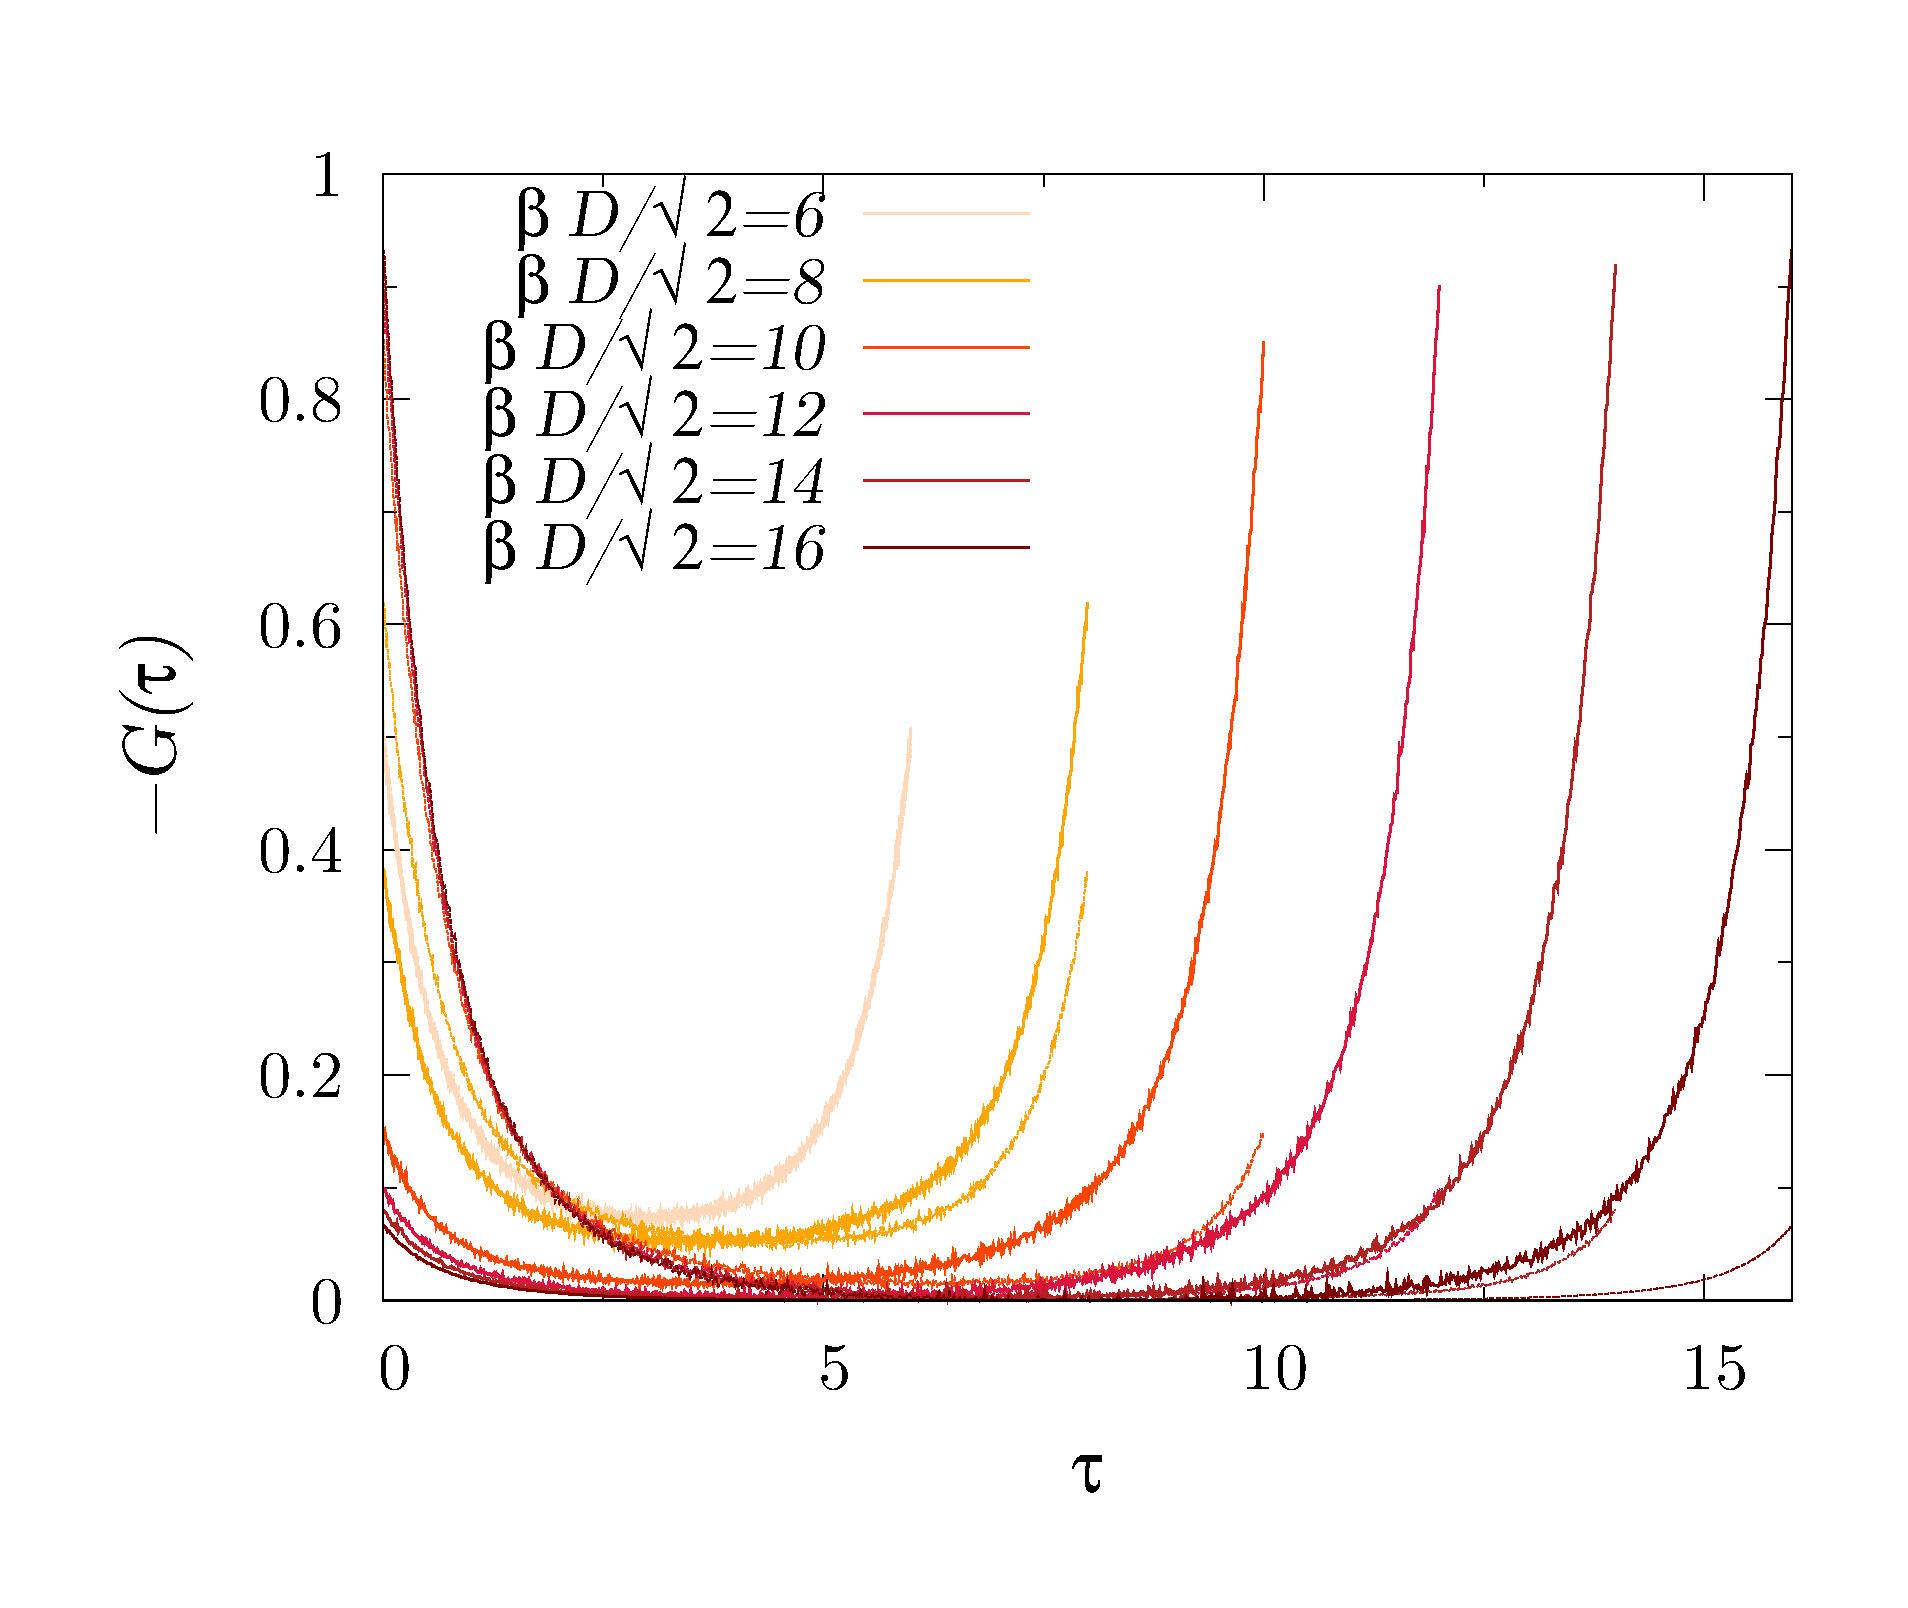
\includegraphics[width=0.9\columnwidth]{green.eps}
\caption{(Color online)
Green's functions $G_{\uparrow}$ (solid line) and $G_{\downarrow}$
(dashed line) in the temperature range $\beta D/\sqrt 2 =6,8,...,16$
(from bright to dark lines) for the half-filled Hubbard model
simulated using the CT-HYB impurity solver and a DMFT self-consistency allowing for antiferromagnetic order.  
}
\label{fig:hyb1}
\end{figure}
We present here two examples that illustrate the power of these methods and show how they may be used in practice. Further examples and tutorials are available online. First we show the example of a paramagnetic metal being cooled below the N\'{e}el temperature $T_{\rm N}$ and developing antiferromagnetic correlations -- an example taken from Fig.~11 of Ref.~\cite{Georges96}. Secondly we illustrate the lack of discretization errors in continuous-time algorithms by comparing self-energy data to Fig.~$15$ in the same publication (see also Fig.~$4$ in Ref.~\cite{Gull08_ctaux}). Both examples are available as tutorials in the ALPS package available at \href{http://alps.comp-phys.org}{http://alps.comp-phys.org}, along with detailed instructions on how to install programs and libraries and how to run the simulations. 
%In order to get started with the two continous-time quantum impurity solvers published in this paper we will present examples for a single-site DMFT calculation. For this purpose we will consider the paramagnetic to antiferromagnetic transition in the half-filled Hubbard model on the Bethe lattice. 
\subsection{N\'{e}el transition in single site DMFT}
We study a single-orbital Hubbard model at an interaction strength $U/D=3 /\sqrt 2$ within the temperature range $\beta D/\sqrt 2 =6,8,...,16$, where $D$ is the half-width of a semi-circular density of states. Because of the simple structure of the Hilbert transform Eq.~(\ref{HilbertSemi}) and the exact limit of infinite coordination number such examples are frequently used to test the dynamical mean-field theory and benchmark algorithms. 
We measure the imaginary-time Green's function $G_{\sigma}(\tau)=-\langle \mathcal{T}_{\tau} c_\sigma(\tau)c_\sigma(0)^\dagger \rangle$ and show results for spin $\sigma=\uparrow$ and $\sigma=\downarrow$ in Fig.~\ref{fig:hyb1}. The value $-G(\tau = \beta)$ corresponds to the expectation value of the occupation number $n_{\sigma}$. For $\beta D/\sqrt 2 =6$ the system is in a paramagnetic phase and hence $n_\uparrow = n_\downarrow = 1/2$. Upon reducing temperature ($\beta D/\sqrt 2 =8,...,16$) the occupation numbers for `up' and `down' spins $n_\uparrow$, $n_\downarrow$ start to deviate as the system enters the antiferromagnetic phase. 
For $\beta D/\sqrt 2 =16$ a self-consistent solution is reached within 10 iterations, typical runtimes on current computers are on the order of two minutes.
In the ALPS package we provide a python script to run the example presented, which can be found in the tutorial DMFT-02 CT-HYB. The simulation is started by running \verb*#vispython tutorial2a.py# in a terminal.


\begin{figure}
\includegraphics[width=0.9\columnwidth]{se}
\caption{
(Color online) Self-energy for the paramagnetic dynamical mean-field solution of the half-filled Hubbard model with interaction strength $U/t = 4.24$, at inverse temperature $\beta =22.64/t$. Data reproduced from Fig. 15 of Ref.~\cite{Georges96} (ED, HF) and from Fig.~4 of Ref.~\cite{Gull08_ctaux} (CT-AUX). Shown are Hirsch Fye data with discretization (``Trotter'') errors for different values of $\Delta \tau$, as well as accurate exact diagonalization (\cite{Caffarel94}) data converged in the number of bath sites and data from the numerically exact algorithms CT-HYB, CT-AUX and CT-INT. The continuous-time and ED data are indistinguishable.
\label{fig:sigma}
}
\end{figure}
\subsection{Paramagnetic metal and extrapolation errors}
To illustrate one of the main advantages of continuous-time algorithms, the absence of discretization errors, we show results for the self-energy of a weakly interacting paramagnetic metal at low temperature in Fig.~\ref{fig:sigma}.
This is a regime of parameter space that is well described by Fermi liquid theory. Unlike in the Hirsch-Fye algorithm, discretization errors are not present and the results are very well consistent with results from e.\,g. exact diagonalization (see Ref.~\cite{Georges96}, Fig. 15), which may be considered to be exact for this problem.
Fig.~\ref{fig:sigma} can be generated by executing \verb*#vispython tutorial6a.py# for CT-HYB and  \verb*#vispython tutorial6b.py# for CT-INT of `Tutorial DMFT-06 Paramagnet' and plotting the self energy files of the last DMFT-iterations.


We would like to direct the reader's attention to further examples and tutorials on the ALPS Project website \cite{ALPS}.

\section{Acknowledgments}
E.~G. is supported by NSF under Grant No.~DMR-0705847 and P.~W. by the Swiss National Science Foundation (grant PP002-118866). T.~P. and S.~F. acknowledge support by the Deutsche Forschungsgemeinschaft through the collaborative research center SFB~602 and by the PPP exchange program of the German Academic Exchange Service (DAAD).
We gratefully acknowledge support by the wider ALPS community.

\bibliographystyle{apsrev4-1}
\bibliography{refs_shortened.bib}

\end{document}

